
Tuscarora is a framework for developing and deploying multiple networking patterns in heterogeneous MANETs.
This manual explains how to install and use Samraksh's Tuscarora framework. 
%This version (v1.0) is the first stable
%release of the framework, thus the APIs are likely to %continue to evolve.

\section{Definitions}

\begin{description}
\item [API:] Short for Application Programming Interface. In our case
  this refers to a single publicly accessible method defined in a
  class. When referring to multiple methods it will be used in plural
  as APIs or as an Interface.

\item [Interface:] A set of publicly accessible methods defined in a
  class. An interface is usually defined as a pure abstract class
  that needs to be implemented by some class before it can be
  instantiated.

\item [Neighbor:] Node k is a neighbor of node j if a request to send
  a datagram from j to k could be directly acted upon and is expected
  to succeed in a single hop. A neighbor is identified by an
  identifier assigned independently by Tuscarora to that neighbor.
  That identifier has type \CPPClassName{NodeId\_t}, which is a 16-bit unsigned integer;
  it is sometimes called the ``node ID'' of the neighbor.  Note that the
  identifiers assigned to neighbors have strictly local scope.  In
  particular, different neighbors of the same node may know it by
  different node IDs. 

\item [Neighborhood:] The neighborhood of a node is the set of
  current neighbors of that node.

\item [Waveform Name:] An identifier that is assigned independently
  by the framework to uniquely identify each waveform on the
  device. Colloquially this might be referred to as the Waveform ID.

\item [Link:] The ordered pair consisting of the Neighbor ID and
  Waveform ID of a waveform that is expected to be valid for reaching
  that neighbor. Simply put, it is a combination of the node ID and the
  waveform ID.  The same Node ID may occur in multiple links, if a
  neighbor is reachable via more than one waveform.

\item [Link Metrics:] A measure of the performance, quality, or other
  property of a link that is sufficiently standardized that it may be
  used by patterns to compare the link with other links over
  potentially different waveforms. Please see Section
  \ref{Sec:Metrics} for more details.
\end{description}

\section{Target Audience}
This document is intended for developers who use the
Tuscarora Framework to write applications, new Networking Patterns or to develop
Waveforms that would be compatible with the framework. If you would
like to understand the design rationale of the framework, please read
the ``Tuscarora Framework Design'' document. If you are a Waveform
developer you should also consult the ``Waveform Interface
Definitions'' document.

\section{Deployment Targets}

The current version of the framework can be built and run only on the
NS3-DCE simulation system as well as on any standard POSIX/Linux systems. 
The architecture allows flexibility as it allow single-process and multi-process setups depending on the platform requirements. 
The details of  how to configure different types of builds and the associated binding requirements will be elaborated in \cref{Chap:ILS}.

\section{Tuscarora Framework Overview}

Tuscarora is Framework for building scalable heterogeneous MANETs. The
framework is designed to support many simultaneous instances of what would
traditionally be called routing protocols, which we refer
to as `Application-Specific Networking Patterns' (ASNPs) or 'Network Patterns' or even simply as `Patterns'. The core service provided by the framework is a
Standardized Neighborhood Abstraction. Tuscarora framework design is influenced by Samraksh's work on DARPA's Fixed Wireless At a Distance program. 

\begin{figure}[ht]
 \centering
 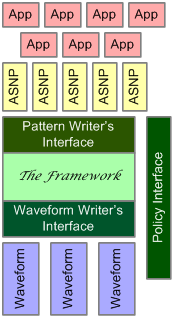
\includegraphics{figures/ASNPContext}
 \caption{Framework Design Goal}
 \label{Fig:Goal}
\end{figure}

Figure~\ref{Fig:Goal} shows the notional architecture of the
framework. Tuscarora is designed to support these broad goals:  
\begin{itemize}
 \item Scaling of MANETs: By supporting multiple patterns and even
   multiple instances of a Pattern, an application will be able to
   choose a pattern that closely matches its data distribution needs,
   thereby decreasing overhead significantly versus the traditional
   any-to-any routing approach.

 \item Portability: A standardized abstraction for Patterns makes them
   portable across platforms and waveforms.

 \item Support Heterogeneity: Standardized abstractions for waveforms
   allow any waveform that implements the abstractions to be ``plugged
   in'' to the framework.  Moreover, every Tuscarora node is a ``gateway''
   node between all supported waveforms.

 \item Flexible Management: An open policy manager that operates on
   self-describing management interfaces of modules provides a very
   flexible way of managing the network.  Further, it enables a
   human-in-the-loop management architecture to carry out network and
   mission management tasks.
\end{itemize}

To understand the design decisions better, please see the Tuscarora
Design Rationale document.

\subsection{Services}
\label{Subsec:Services}

To accomplish the foregoing goals, the framework provides the following services:
\begin{itemize}
 \item \textbf{Neighborhood service:} Discovers neighbors and evaluates the
   quality of their links; notifies Patterns (via callbacks)
   whenever there are changes in the neighborhood.

 \item \textbf{Data Flow:} Provides multi-destination send and broadcast
   services; also provides various forms of notification (acks) when messages
   are sent out and/or received at the destination.

 \item \textbf{Pattern Naming:} Provides a way of naming patterns. Multiple
   instances of the same pattern can be instantiated in the network.

 \item\textbf{ Policy Manager:} Implements a number of policies for the framework. Also provides hooks for a network manager to various other modules which might support policy definitions.
\end{itemize}


The developers of the framework have also defined a number of optional services, that might be useful or even necessary on some platforms.
These are not standardized and are not expected to be available on all platforms. Samraksh is not responsible for providing these services, however
we might provide this service as a library or specific implementations for some platforms.
\begin{itemize}
	\item \textbf{Time Stamping:} This service provides timestamps for events.  The basic idea of this service is to translate a event that happened on a (direct) neighboring node to a corresponding time on a given node. That is provide a basis for synchronization of times when time synchronization is not available already.
	Two variations are defined a explicit sender based and implicit receiver based. In the explicit sender based version, a sending node marks a Event Time, in some time unit, puts it into a packet and sends it to a neighbor. The receiver node takes a timestamp when this packet is received on the lower levels. If the delays between the sending node taking the timestamp and the receiver node taking its timestamp can be accomplished then the event times across the two nodes can be  synchronized. In implicit receiver based timestamping, the sending part is absent. The receiver is expected to know the rate or schedules  at which an packet sending event is supposed to happen on a neighbor and simply expects packets according to that schedule. The implicit timestamping service simply takes a timestamps of all incoming packets and sends them to the user of the service which can then parse these timestamps to arrive at time mapping between the two nodes.
	
	\item \textbf{Neighbor Time:} This services provides a given neighbor's time corresponding to local time. This is also called as network time synchronization service. This is expected to build on top of the timestamping service. However, specialized radios/waveforms may be able to implement this all by themselves.
	
	\item \textbf{Location:} Provides the geographical coordinates of a node. This service will need to interface with some underlying hardware such as GPS or location systems.
	
	\item \textbf{Mobility Control:} Provides the ability to move the current node to a given location or set the motions towards a given direction. Useful for nodes that can move or for mobile simulations.
	
	\item \textbf{ Global Name}: Provides a globally unique name for a node. Patterns or Apps might query this service to get a the nodes global name and use it as the identifies in its protocols and algorithms.
	
\end{itemize}


\subsection{List of Key Interfaces}

List of APIs:
\begin{itemize}
 \item  Implemented by platform Shim Layer provider
    \begin{itemize}
      \item PatternBase
      \item FrameworkShim
    \end{itemize}
 \item Implemented by Framework provider (Accessible by the Patterns)
    \begin{itemize}
      \item Framework\_I
      \item PatternNaming\_I
      \item PatternNeighborTable\_I (As a library)
    \end{itemize}
 \item Implemented by the Waveforms
    \begin{itemize}
      \item Waveform\_I
      \item WF\_LinkEstimator\_I
    \end{itemize}
\end{itemize}


List of Service APIs:
\begin{itemize}
 \item Implemented by Framework
    \begin{itemize}
      \item LinkEstimation\_I
      \item PotentialNeighborRegistry\_I
      \item NetworkDiscovery\_I (default)
      \item PolicyManager\_I
      \item NeighborTable\_I
      \item PatternNaming\_I
    \end{itemize}
 \item Implemented by external providers
    \begin{itemize}
      \item GlobalNodeName\_I
      \item LocationService\_I
      \item NeighborTime\_I
      \item NetworkDiscovery\_I (Overrides the default if available)
   \end{itemize}
\end{itemize}